\subsection{Introduction}
\begin{frame}{Train and Prediction Errors}
  \begin{itemize}
  \item Loss-function \(L(y, \hat{y}) = 0 \text{ if } y=\hat{y} \text{ else } 1\)
    
  \item \textbf{Train error}: average loss over the training sample
    \begin{eqnarray*}
      \text{Err}_{\text{train}} = \frac{1}{n}\sum_{i=1}^nL(y_i, \hat{y}_i)
    \end{eqnarray*}
  \item \textbf{Test/Prediction error}: average loss over an independent test sample \(\to\)  \structuretext{Generalization error}
    
  \item General picture:  
    \begin{eqnarray*}
      \text{Err}_{\text{test}} \approx \text{Err}_{\text{train}}  + O
    \end{eqnarray*}
    \(O\) would be the average \emph{optimism}.
  \end{itemize}  
\end{frame}

\begin{frame}{Model Selection vs Model Assessment}
  \begin{block}{Model selection}
    \begin{itemize}
    \item Estimate the best set of hyperparameters
    \item Estimate the performance of differents models
    \end{itemize}    
  \end{block}

  \begin{block}{Model Assessment}
    Estimate the generalization error on unseen/test sample    
  \end{block}
  \vspace{1cm}
  
  \visible<2>{
    \begin{center}
      \begin{tabular}{*6{p{5em}}}
        \multicolumn{6}{c}{$\longleftarrow$ Total Number of Dataset $\longrightarrow$}\\
        \cellcolor{orange} Train & \cellcolor{orange} Train & \cellcolor{orange} Train & \cellcolor{orange} Train & \cellcolor{orange} Train & \cellcolor{green} Validation       
      \end{tabular}
    \end{center}

  }  
\end{frame}

\subsection{Cross-validation}
\begin{frame}{Principle}
  \begin{itemize}
  \item Method to estimate prediction error using the training sample
  \item Based on splitting the data in \(K\)-folds :    
    \begin{center}
      \begin{tabular}{l*5{p{5em}}}
        Model 1 & \cellcolor{orange} Train & \cellcolor{orange} Train & \cellcolor{orange} Train & \cellcolor{orange} Train & \cellcolor{green} Validation \\
        Model 2 & \cellcolor{orange} Train & \cellcolor{orange} Train & \cellcolor{orange} Train & \cellcolor{green} Validation & \cellcolor{orange} Train \\
        Model 3 & \cellcolor{orange} Train & \cellcolor{orange} Train & \cellcolor{green} Validation & \cellcolor{orange} Train & \cellcolor{orange} Train \\
        Model 4 & \cellcolor{orange} Train & \cellcolor{green} Validation & \cellcolor{orange} Train & \cellcolor{orange} Train & \cellcolor{orange} Train \\
        Model 5 & \cellcolor{green} Validation & \cellcolor{orange} Train & \cellcolor{orange} Train & \cellcolor{orange} Train & \cellcolor{orange} Train 
      \end{tabular}
    \end{center}
    
  \item Expected prediction error:
    \begin{eqnarray*}
      CV(\hat{f},\theta) = \sum_{k=1}^K\text{Err}_k(\hat{f},\theta)
    \end{eqnarray*}
  \end{itemize}
\end{frame}

\begin{frame}{Pratical advices}
  \begin{itemize}
  \item K ? Usually K=5 or 10 is a good trade-off (K=n is called leave-one-out)
    \begin{center}
      \begin{tabular}{ccc}
        \toprule
        &Bias & Variance \\
        \midrule
        K low & High & Low \\
        K high & Low & High \\
        \midrule
        K = n & Low & Very High \\
        \bottomrule
      \end{tabular}
    \end{center}
  \item Be careful to the learning curve
    \begin{center}
      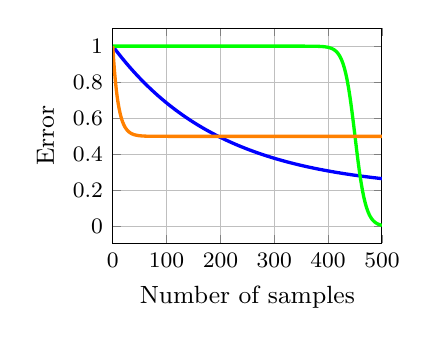
\begin{tikzpicture}
        \begin{axis}[domain=0:500,samples=300,footnotesize, grid,xlabel={Number of samples}, ylabel={Error}, xmin=0,xmax=500]
          \addplot[mark=none, blue, very thick] {0.8*exp(-x/200)+0.2};
          \addplot[mark=none, green, very thick] {1- 1/(1+exp(-(x-450)/10))};
          \addplot[mark=none, orange, very thick] {0.5*exp(-x/10)+0.5};
        \end{axis}
      \end{tikzpicture}
    \end{center}
  \item Model should be trained completely for each fold (i.e., data normalization, optimization, etc \ldots)
  \item \alert{Notebook}
  \end{itemize}  
\end{frame}
%%% Local Variables:
%%% mode: latex
%%% TeX-master: "main"
%%% End:
